\begin{frame}{RTDroid - Broadcast Channel}
	\only<2>{\centering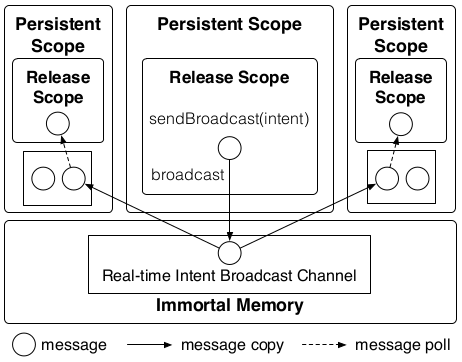
\includegraphics[scale=0.40]{broadcastChannel}}
	\only<1>{\begin{itemize}
		\item Simile ai canali punto a punto, ma in broadcast
		\item Un contatore mantiene il numero di riceventi in attesa
		\begin{itemize}
			\item Conosciuto staticamente grazie a \texttt{manifest.xml}
		\end{itemize}
		\item Messaggio salvato nella memoria immortal e liberato quando tutti lo hanno ricevuto
		\item Utilizzo di memoria limitato e non soggetto a GC
		\begin{itemize}
			\item Nessuna fonte di interferenza
		\end{itemize}
	\end{itemize}}
\end{frame}